\chapter{\MediK{}: Towards Safe Guidelines-based \CDSSs{}}\label{chapter:medik-safe-cdss}

In \autoref{chapter:k-based-guidelines}, we discussed the process
of encoding best practice guidelines (\BPGs{}) as \K{} definitions
to describe a systematic way of building \CDSSs{}. Specifically,
we described the process of encoding medical knowledge in guidelines
notionally via workflows that can be expressed abstractly as
concurrently executing finite state machines that communicate
via passing messages. Next, we described the process of
expressing state machines as \K{} definition, where \K{} features
such as configuration abstraction and local rewriting
enable \emph{conciseness}. We then combined the \K{} definition
with a simple javascript-based frontend to develop a \CDSS{}
for assisting healthcare practitioners (\HCPs{}) follow the
Advanced Life Support (\ALS{}) guidelines for managing
cardiac arrest published by the American Heart Association.

In \autoref{chapter:hurdles-cdss-adoption}, we described
that wider \CDSS{} adoption is incumbent on a having a
systematic way of developing guidelines with validated
content. The approach described in \autoref{sec:semantics-first}
attempts to enable such a way. It dictates that:
\begin{enumerate*}[label=(\roman*)]
  \item the semantics of the language be formally defined, from
  which tools are derived from a correct-by-construction fashion, and,
  \item ensuring that semantics of medical knowledge is accurately
  described.
\end{enumerate*}
As is typically the case, the \KACLS{} system from
\autoref{sec:kacls-cdss} through collaboration between
\HCPs{} and computer scientists. While the \K{}-based
representation of the \ALS{} guideline was concise,
it was not easily comprehensible to \HCPs{}, or to other
software engineers without prior experience of using \K{}.
This chapter addresses limitations of our work from
\autoref{chapter:k-based-guidelines}. Specifically, we describe
\MediK{} (pronounced \say{Medi-kay} \footnote{\MediK{} is a portmanteau of
Medicine and \K}) a novel domain-specific language (\DSL{}) for
expressing medical knowledge that is designed from the ground-up
with \HCP{}-comprehensibility in mind. As the name suggest, \MediK{}
has a formal $\K$ semantics, from which all tools for it are derived,
including its interpreter. \MediK{} has been used to implement a
complex \CDSS{} for management of sepsis in pediatric cases that
has multiple concurrent workflows. Our \MediK-based system has
been shown to satisfy desired safety properties, and to the
best of our knowledge, is the first such system with formal safety
guarantees.

The rest of this chapter is organized as follows. In \autoref{sec:sepsis-bpg}
we recall the example \BPG{} from section \autoref{sec:bpg-background}
for management of sepsis, to illustrate common requirements
that \DSL{} for modeling \BPGs{} should satisfy.
In \autoref{sec:medik}, we introduce the \MediK{} \DSL{}, and illustrate how
it has been specifically designed to address said requirements.
In \autoref{sec:evalution}, we evaluate the effectiveness of our approach
by utilizing it to build a \CDSSs{} intended for real-world use.
In section \autoref{sec:discussion}, we discuss how \MediK{} builds on
existing approaches in \autoref{chapter:related-work} to advance the
tate-of-art in addressing challenges from \autoref{chapter:hurdles-cdss-adoption}.


\section{Pediatric Sepsis Management \BPG{}}\label{sec:sepsis-bpg}

In \autoref{sec:bpg-background}, we presented a best practice
guideline for management of sepsis in pediatric cases.
We briefly describe the guidelines here. Recall that
sepsis is life-threatening condition caused by the body's extreme response to
an infection, and is a major cause of morbidity and mortality
in children. Evidence indicates that timely
identification and prompt treatment with antibiotics and
intravenous (IV) fluids is \emph{vital} for avoiding
adverse outcomes \cite{Weiss2014CCM,Evans2018JAMA}.
The \BPG{} has several concurrent workflows with inter-workflow
dependencies, making it suitable to study common characteristics of \BPGs{},
which we recall here. Specifically, \BPGs{}:
\begin{itemize}
  \item Involve \stress{concurrent} workflows, such as administering drugs,
    monitoring vitals, performing treatment, etc. There may also be
    inter-workflow interactions. For instance, a diagnosis of sepsis during the
    screening may require modifications to an ongoing course antibitiotics.
  \item Often specified in a \stress{flowchart-like}
    notation. See \cite{AHAFlowcharts} and \cite{CancerCareFlowcharts} for other flowchart-based \BPGs{} for management of \emph{cardiac arrest}, and
    screening, risk-reduction, treatment and survivorship in
    cancer care respectively.
  \item Require communication between \stress{heterogeneous agents} such as
     monitors and Electronic Health Records (EHRs).
  \item Often use \stress{tables} indexed by parameters such as age, weight,
    etc to present normal/abnormal ranges for measurements, or recommended dosages for drugs.
\end{itemize}
%While section
%\autoref{sec:bpg-background} briefly discussed some sepsis workflows, here
%we discuss remaining workflows and their interdependencies in detail.

%Recall from \autoref{sec:bpg-background} that once sepsis has been detected,
%it is treated by administering fluids and antibiotics.
%Additionally, sepsis
%lead to septic shock---a condition characterized by acute cardiovascular
%distress.

%Adverse outcomes can, however, be mitigated through timely
%identification and prompt treatment with antibiotics and
%intravenous (IV) fluids \cite{Weiss2014CCM,Evans2018JAMA}.
%\BPGs{} for screening and management of sepsis in pediatric Emergency
%Departments (EDs) have shown effectiveness in screening and management of sepsis \cite{Eisenberg2021JP},
%leading to their adoption in many pediatric EDs \cite{Balamuth2017EM,Sepanski2014FP}.
%
%In \figurename{} \ref{fig:sepsis-screening}, we present a simplified version of
%the screening section of OSF's sepsis mangement guideline.
%In essence, when a patient arrives at the
%\ED{} with a fever or an infection, the \HCP{} is supposed to obtain
%\begin{enumerate*}[label=(\alph*)]
%  \item the patient's age,
%  \item any conditions, such as cancer, immunosuppresssion, etc,
%    that increase likelihood of sepsis, and
%  \item the patient's vital signs, such as heart rate, systolic blood
%    pressure, respiratory rate, etc.
%\end{enumerate*}
%\begin{footnotesize}
%  \begin{table}
%    \centering
%    \begin{tabular}{ | c || c | c | c | }
%      \hline
%      \textbf{Age}            & \textbf{Heart Rate}   & \textbf{Systolic BP} & \textbf{Temp}  \\
%      \hline
%      $0d - 1m$               & $>205$                & $<60$                & $<36 \text{ or } >38$ \\
%      \hline
%      $\geq 1m - 3m$          & $>205$                & $<70$                & $<36 \text{ or } >38$ \\
%      \hline
%      $\geq 3m - 1y$          & $>190$                & $<70$                & $<36 \text{ or } >38.5$ \\
%      \hline
%      $\dots$                 & $\dots$               & $\dots$              & $\dots$ \\
%      \hline
%      $\geq 13y$              & $>100$                & $<90$                & $<36 \text{ or } >38.5$ \\
%      \hline
%    \end{tabular}
%    \caption{Vital Signs Chart}\label{table:vital-signs}
%  \end{table}
%\end{footnotesize}
%
%This information is then used to check for abnormalities
%in clusters of linked information, called \say{buckets}. For instance, if
%the patient's heart rate is abnormal, then \say{bucket 1} is said to
%have an abnormal value.
%Checking for such abnormalities often involves the use of tables, such as
%\tablename{} \ref{table:vital-signs} that contains normal ranges indexed by
%\emph{age}.
%%\footnote{For brevity, we omit some age ranges and vital signs from table
%%\ref{table:vital-signs}}.
%If the patient has at least one abnormal value in every \say{bucket},
%then he/she is flagged as potentially septic.
%
%The \BPG{}-recommended treatment for
%sepsis involves multiple concurrent workflows, such as
%screening for septic shock, fluid resuscitation, and administering antibiotics.
%In \figurename{} \ref{fig:fluid-therapy}, we provide
%a version of the fluid resuscitation guideline used
%at OSF. Briefly, if the patient is flagged as potentially septic, the guideline suggests
%\begin{enumerate*}[label=(\roman*)]
%  \item obtaining any fluid-overload risks,
%  \item administering normal saline (typically over a period of 15 minutes),
%    where the dosage is dictated by risks determined in previous step,
%  \item assessing signs of fluid-overload,
%  \item evaluating patient responsiveness to normal saline upon completion of
%    the administering process, and,
%  \item determining whether another fluid bolus should be administered based on
%    information from previous steps.
%\end{enumerate*}
%\begin{figure}[b]
%  \centering
%  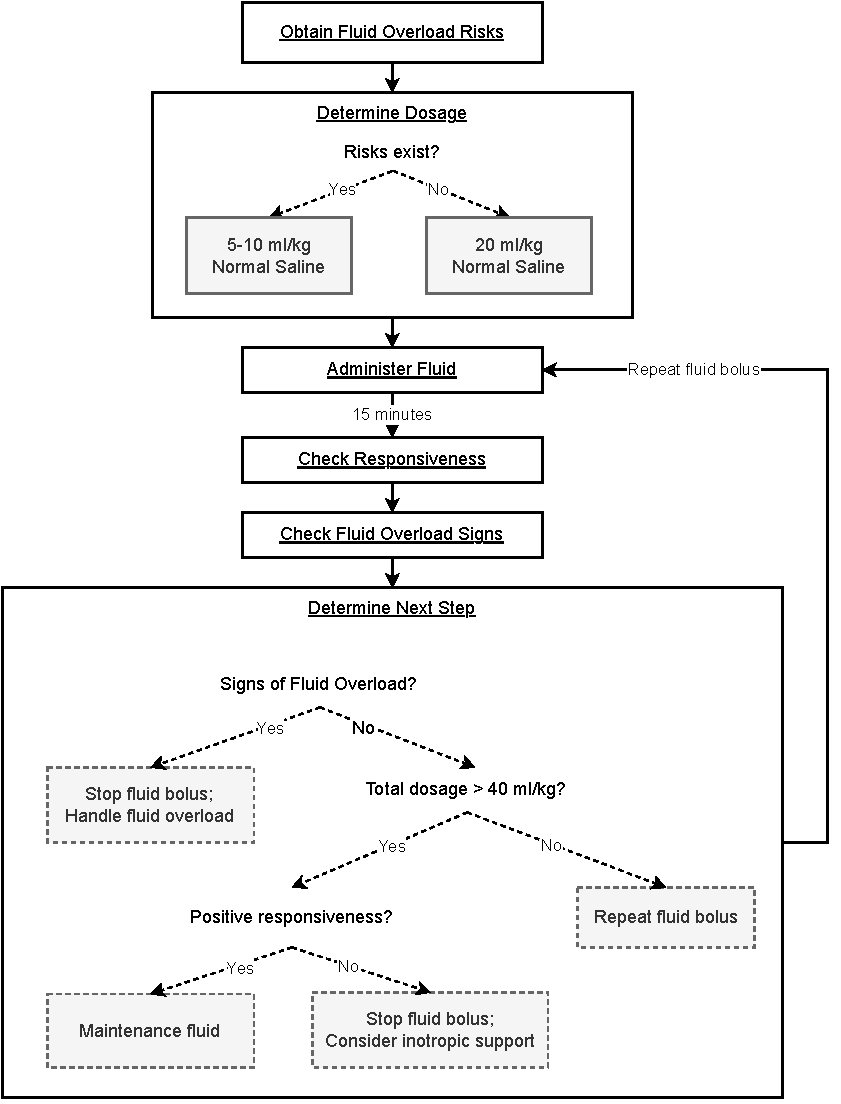
\includegraphics[scale=0.45]{FluidWorkflow-fmcad.pdf}
%  \caption{Fluid Resuscitation Guideline}\label{fig:fluid-therapy}
%\end{figure}
%
%This real-world \BPG{} exhibits characteristics common
%across many \BPGs{}. Specifically \BPGs{} typically:
%\begin{itemize}
%  \item Involve \stress{concurrent} workflows, such as administering drugs,
%    monitoring vitals, performing treatment, etc. There may also be
%    inter-workflow interactions. For instance, a diagnosis of sepsis during the
%    screening may require modifications to an ongoing course antibitiotics.
%  \item Often specified in a \stress{flowchart-like}
%    notation. See \cite{AHAFlowcharts} and \cite{CancerCareFlowcharts} for other flowchart-based \BPGs{} for management of \emph{cardiac arrest}, and
%    screening, risk-reduction, treatment and survivorship in
%    cancer care respectively.
%  \item Require communication between \stress{heterogeneous agents} such as
%     monitors and Electronic Health Records (EHRs).
%  \item Often use \stress{tables} indexed by parameters such as age, weight,
%    etc to present normal/abnormal ranges for measurements, or recommended dosages for drugs.
%\end{itemize}
%
%Note that the aforementioned characteristics are \emph{not} specific
%to one guideline. According to a review paper on \CIGs{} \cite{ClerqAIM03},
%such \DSLs{} should additionally
%\begin{enumerate*}[label=(\alph*)]
%  \item be formally defined, i.e, have a formal syntax and semantics, and
%  \item have an execution engine to provide decision support.
%\end{enumerate*}

In the following sections, we describe how these characteristics dictate the
design philosophy behind \MediK{}. We argue that this philosophy
makes \MediK{} both intuitive to \HCPs{}, and suitable for expressing
complex guidelines.

\section{Design Considerations}\label{sec:medik}

This section introduces the \MediK{} \DSL{} through its $\K$
syntax and semantics.
We developed $\MediK{}$ to realize
the semantics-first approach discussed in \autoref{sec:semantics-first}.
Thus, it has:
\begin{itemize}
  \item A formally defined, unambiguous semantics.
  \item A correct-by-construction interpreter derived from the semantics.
    As discussed in \autoref{chapter:evaluating-k},
  \item A comprehensive suite of formal program analysis tools.
  \item The ability to quickly adapt physician feedback, as only the semantics
    need to be changed an all tools evolve automatically.
\end{itemize}

The remainder of this section introduces the \MediK{} \DSL{}, and describes how it's
designed to accommodate characteristics of \BPGs{} discussed in
\autoref{sec:bpg-background}.

\subsection{\HCP{} Comprehensibility}

\begin{lstlisting}[
  float=b!,
  frame=single,
  style=mediksty,
  language=medik,
  numbers=left,
  numbersep=5pt,
  numberstyle=\tiny,
  caption={Skeleton of a \MediK{} Machine},
  label={lst:machine-skeleton},
  xleftmargin=3ex
]
[init] machine <IDENTIFIER>                     @\label{lstline:machine-declaration}@
  receives <IDENTIFIER_LIST> {                  @\label{lstline:machine-receives}@
  vars <IDENTIFIER_LIST>;                       @\label{lstline:global-declarations}@

  [init] state <IDENTIFIER> {                   @\label{lstline:state-block-start}@
    entry [(IDENTIFIER_LIST)] {                 @\label{lstline:entry-block-start}@
      <STMT> // entry block
    }                                           @\label{lstline:entry-block-end}@
    on <IDENTIFIER> [(IDENTIFIER_LIST)] do {    @\label{lstline:handler-block-start}@
      <STMT> // event handler
    }                                           @\label{lstline:handler-block-end}@
  }                                             @\label{lstline:state-block-end}@
}
\end{lstlisting}

Our approach stresses that \HCPs{} must be able to comprehend the
guideline, and if necessary, making changes to on their own. As discussed
in \autoref{chapter:hurdles-cdss-adoption}, this has several hurdles, chief
among which is the fact that \HCPs{} are typically not trained to understand
conventionally programming languages. Thus, \HCPs{} need to work collaboratively
to translate the \BPG{} into a computable medium.
In essence, the \BPG{} serves as a functional
specification for implementing the \CDSS{}. But, this may lead to
a gap in the \HCPs{}' understanding of the system, and the actual
behavior.
To address this, we designed \MediK{}
s.t. encoded guidelines resemble their physical, non-executable counterparts,
with the intention that familiarity with non-executable guidelines
would also translate to computable \MediK{} ones.

Recall from \autoref{sec:generic-bpg} that \BPGs{}
typically involve concurrent workflows,
often expressed using a flowchart-like notation that may involve
inter-workflow interactions. In \autoref{sec:kacls-backend},
we discussed the merits and suitability of concurrently executing
state machines for modeling medical guidelines.
Thus, we looked at state-of-art languages for modeling large concurrent
systems using state machines, such as P \cite{DesaiPLDI13}, but made
adaptions to make expressing \BPGs{} easier.

In \MediK{}, like in P, programs are expressed as concurrently
executing instances of state machines that communicate via passing messages.
Given a \BPG{} where each workflow is expressed as a flowchart,
we express said flowcharts as State Machines in \MediK{}. Each flowchart node
in the \BPG{} is represented as a state in a state machine, and
edges are represented as state transitions. During execution,
instances of these machines are created, which interact with each other by
passing events. Note the distinction between
machine and its instance. A machine
is analogous to an Object Oriented Programming (OOP) class, whereas
its instance is analogous to an OOP object.


%We achieve this by defining \MediK{} (i.e., its syntax and semantics) in $\K$.
%$\K{}$ is a rewriting-based framework for defining executable
%semantics of languages, type systems and formal analysis tools.
%It has been successfully used to define executable semantics
%of many real world languages such as C \cite{HathhornPLDI15}, Java
%\cite{BogdanasPOPL15}, Javascript \cite{ParkPLDI15}, and the
%Ethereum Virtual Machine \cite{HildenbrandtCSF18}.
%We will introduce $\K$ by need while discussing \MediK{}. For more details on
%$\K$, we refer the reader to \cite{SerbanutaETNCS14} \cite{RosuJLAP10}.
%Once the executable
%semantics of a language have been defined in $\K{}$, it provides us with
%suite of tools such as an interpreter, deductive-verifier and a
%model-checker as shown in \figurename{} \ref{fig:k-overview}.

%The $\K{}$ ecosystem provides a suite of tools, such as an interpreter,
%model-checker, and deductive verifier that are parametric over the language's
%semantics, as shown in \figurename{} \ref{fig:k-overview}. Thus, by
%defining the semantics of \MediK{} in $\K{}$, we obtain aforementioned
%tools for it without any extra effort. Additionally:
%\begin{itemize}
%  \item The $\K$-based interpreter for \MediK{} essentially executes the language's
%    semantics rules, it is correct-by-construction.
%  \item Incorporating changes to \MediK{} only requires updating
%   the semantics. Since the tools are derived from the semantics,
%   they're automatically updated.
%\end{itemize}


%The remainder of this section introduces \MediK{} and describes
%how it's designed around characteristics of \BPGs{} from Section \ref{sec:motivating-example}.
%Recall that \BPGs{} typically involve concurrent workflows, often expressed using a
%flowchart-like notation that may involve
%inter-workflow interactions. To ensure \MediK{} programs are comprehensible
%to \HCPs{}, they must be representable in a flow-chart like notation that \HCPs{}
%are already comfortable with, and be capable of expressing inter-workflow
%interactions succinctly. To address these requirements, we borrow from
%from existing state-of-art languages for modeling large concurrent
%systems, like P \cite{DesaiPLDI13}, but make adaptions to make expressing and
%validating \BPGs{} easier. We explore the differences
%to existing techniques in section \ref{sec:related-works}.

Next, we describe \MediK{} using its $\K$-framework definition.
Recall from \autoref{sec:semantics-in-k}, the $\K{}$ definition
of a language has two components. The first is the language's
syntax, which is defined using a BNF-like notation. $\K{}$
utilizes this grammar to generate a parser for program in the language. We
describe \MediK{}'s syntax in depth in Section \ref{sec:syntax}.
The second is the semantics, which is defined using a $\K{}$-configuration and
rewrite rules. The $\K{}$-configuration
organizes the program's execution state. Rewrite rules
that operate over said configuration dictate the evolution
of program state during execution.
We describe the semantics in greater depth in Sections
\ref{sec:configuration} and \ref{sec:rules}\footnote{The complete executable semantics is available at
 \cite{medikUrl}.}

\section{\MediK{} Syntax}\label{sec:syntax}

\begin{lstlisting}[
  float=b!,
  frame=single,
  style=ksty,
  basicstyle=\ttfamily\small,
  language=k,
  numbers=left,
  numberstyle=\tiny,
  xleftmargin=3ex,
  caption={\MediK{} Expressions Syntax},
  numbersep=5pt,
  label={lst:medik-exp-syntax}
]
syntax StandaloneExp
                ::= "new" Id "(" Exps ")"                     [strict(2)] @\label{lstline:new-syntax}@
                | "createFromInterface" "(" Id "," String ")" [strict(2)] @\label{lstline:create-from-interface-syntax}@
                | Id "(" Exps ")"                             [strict(2)]
syntax Exp ::= Id                                                         @\label{lstline:value-start}@
             | Val
             | Rat
             | FloatLiteral
             | "this"                                                     @\label{lstline:value-end}@
             | UndefExp
             | "obtainFrom" "(" Exp "," Exp ")" [seqstrict]           @\label{lstline:obtain-from-syntax}@
             | "(" Exp ")"                      [bracket]
             > Exp "." Exp                      [strict(1), left]     @\label{lstline:dot-syntax}@
             > Exp "+" Exp                      [seqstrict, left]     @\label{lstline:exp-syntax-begin}@
             | Exp "-" Exp                      [seqstrict, left]
             | Exp "*" Exp                      [seqstrict, left]
             | Exp "/" Exp                      [seqstrict, left]
             | Exp ">" Exp                      [seqstrict, left]
             | Exp "<" Exp                      [seqstrict, left]
             | Exp ">=" Exp                     [seqstrict, left]
             | Exp "<=" Exp                     [seqstrict, left]
             | "!" Exp                          [seqstrict, left]
             | Exp "&&" Exp                     [strict(1), left]
             | Exp "||" Exp                     [strict(1), left]
             > Exp "==" Exp                     [seqstrict, left]     @\label{lstline:exp-syntax-end}@
             | "interval" "(" Exp "," Exp ")"
             > Exp "in" Exp
             | "parseInt" "(" Exp ")"           [strict]
             | StandaloneExp
\end{lstlisting}


We use the skeleton of a \MediK{} machine in \autoref{lst:machine-skeleton}, and use
it to describe the syntax.
Note that we use \inlinemedik{[...]} to denote
optional constructs, \inlinemedik{<...>} for mandatory constructs, lowercase for
terminals, and uppercase for non-terminals.
%A machine $m = \left(S, E, \Var, s_i\right)$,
%where $S$ is the set of states, $E$ the set of events,
%$\Var$, the set of instance variables, and $s_i$ the initial state.
%As shown in \figurename{} \ref{fig:machine-def}, a typical

\begin{lstlisting}[
  float=ht
  ,style=ksty
  ,language=k
  ,numbers=left
  ,numberstyle=\tiny
  ,numbersep=5pt,
  ,xleftmargin=3ex
  ,caption={\MediK{} Statement Syntax}
  ,label={lst:medik-stmt-syntax}
]
syntax Stmt ::= StandaloneExp ";"                         [strict]
              | "sleep" "(" Exp ")" ";"                   [strict(1)]
              | "send" Exp "," ExtId ";"                  [macro]
              | "send" Exp "," ExtId "," "(" Exps ")" ";" [seqstrict(1, 3)]
              | "broadcast" Id ";"                        [macro]     @\label{lstline:broadcast-stmt-macro}@
              | "broadcast" Id "," "(" Exps ")" ";"       [strict(2)] @\label{lstline:broadcast-stmt-syntax}@
              | "goto" Id ";"                             [macro]
              | "goto" Id "(" Exps ")" ";"                [strict(2)]
              | "print" "(" Exp ")" ";"                   [strict]
              > "return" ";"                              [macro]
              | "return" Exp ";"                          [strict(1)]
              | "var" Id "=" Exp ";"                      [macro]
              > Exp "=" Exp ";"                           [strict(2)] @\label{lstline:assignment-stmt}@
              > "var" Id ";"
              | "vars" Ids ";"                            [macro-rec]
              | Block
              > "if" "(" Exp ")" Block                    [strict(1)] @\label{lstline:if-stmt}@
              | "if" "(" Exp ")" Block "else" Block       [strict(1)] @\label{lstline:if-else-stmt}@
              | "while" "(" Exp ")" Block                             @\label{lstline:while-stmt}@
              | "entry" Block                             [macro]
              | "entry" "(" Ids ")" Block
              | "on" ExtId "do" Block                     [macro]
              | "on" ExtId "(" Ids ")" "do" Block
              | "fun" Id "(" Ids ")" Block
              | NonDetStmt
              | Exp "in" "{" CaseDecl "}"
              | StateDecl
              > "machine" Id Block                        [macro]
              | "machine" Id "receives" Ids Block
              | "interface" Id Block                      [macro]    @\label{lstline:interface-declaration}@
              | "interface" Id "receives" Ids Block                  @\label{lstline:interface-declaration}@
              | "init" "machine" Id Block                 [macro]
              | "init" "machine" Id "receives" Ids Block
              | "yield" ";"
              > Stmt Stmt                                 [right]
\end{lstlisting}

A \MediK{} program consists of a set of machine definitions, where
a machine definition consists of:
\begin{itemize}
  \item (Lines \ref{lstline:machine-declaration}-\ref{lstline:machine-receives})
    The keyword \inlinemedik{machine}, followed by the name
    and a comma-separated list of identifiers signifying events that
    it \inlinemedik{receives} via the broadcast mechanism.
    One state in every machine, and one machine in a program can be
    prefixed with the keyword \inlinemedik{init}. On execution, an implicit instance
    of this machine the created, and the \inlinemedik{entry} block of
    initial state executed.
  \item (\autoref{lstline:global-declarations}) A set of instance variables.
  \item (Lines \ref{lstline:state-block-start}-\ref{lstline:state-block-end}) A set of state declarations. Each
    state has a name, an optional entry block (Lines
    \ref{lstline:entry-block-start}-\ref{lstline:entry-block-end}),
    and a set of event handlers (Lines \ref{lstline:handler-block-start}-\ref{lstline:handler-block-end}).
    The entry block begins with the keyword \inlinemedik{entry}, and may contain a list of variables
    that are bound to values when an instance enters the state during execution.
    One state in the machine may be prefixed with \inlinemedik{init}, specifying the
    initial state that an instance starts execution in.
  \item Event handlers begin with \inlinemedik{on} followed by the event name,
    an optional list of variables bound to data in the event, followed by the
    keyword \inlinemedik{do} a block of the handler's code.
\end{itemize}
%A machine definition starts with the keyword \inlinemedik{machine},
%followed by its name (\autoref{lstline:machine-declaration}). On
%\autoref{lstline:machine-receives}, following the
%\inlinemedik{receives} keyword, is a comma-separated list of identifiers
%signifying the events that the machine can receive from other machines.
%One machine in a program can be
%prefixed with the \inlinemedik{init} keyword. This machine is referred to as the
%initial machine.
%On \autoref{lstline:global-declarations}, following the keyword
%\inlinemedik{vars}, another comma-separeted list of identifiers signifies
%the instance-variables. During execution, each instance maintains a mapping from
%these variables to values. Each machine defines a set of states, such as
%the one in Lines \ref{lstline:state-block-start}-\ref{lstline:state-block-end}.
%A state has a name, an optional entry block
%(\autoref{lstline:entry-block-start}-\autoref{lstline:entry-block-end}),
%and a set of event handlers (Lines
%\ref{lstline:handle-block-start}-\ref{lstline:handler-block-end}). The entry block
%begins with the keyword \inlinemedik{entry}, and may contain a list of variables
%that are bound to values when the state is entered during execution.
%One state in the machine may be prefixed with \inlinemedik{init}, specifying the
%initial state. When execution begins, an implicit instance
%of the initial machine is created, and the \inlinemedik{entry} block of
%its initial state is executed. When an instance of a machine is dynamically
%created during runtime, the \inlinemedik{entry} block of its initial state is executed.
%Event handlers within a state begin with \inlinemedik{on} followed by the event name
%and an optional list of variables. When the event handler is executed, data from
%the received event's payload is bound to aforementioned variables which
%can be used in the code block that follows the \inlinemedik{do} keyword.
%A machine definition consists of:

%\begin{figure}[h]
%  \centering
%\begin{lstlisting}[style=mediksty,language=medik,basicstyle=\ttfamily\scriptsize,numbers=right]
%[init] machine <IDENTIFIER>
%  receives <IDENTIFIER_LIST> {
%  vars <IDENTIFIER_LIST>;
%
%  [init] state <IDENTIFIER> {
%    entry [(IDENTIFIER_LIST)] {
%      <STMT> // entry block
%    }
%    on <IDENTIFIER> [(IDENTIFIER_LIST)] do {
%      <STMT> // event handler code
%    }
%  }
%}
%\end{lstlisting}
%\caption{Machine Definition in \MediK{}}\label{fig:machine-def}
%\end{figure}

Each entry and event handler block contains statements defined
by syntax shown in \autoref{lst:medik-stmt-syntax}. The statements
are written over expressions given by the syntax in
\autoref{lst:medik-exp-syntax}.

Recall from \autoref{sec:semantics-in-k}, in $\K$, productions
are defined using the keyword \inlinek{syntax}, where
terminals are enclosed in quotes (\inlinek{""}), and non-terminals
begin with an upppercase character.

\MediK{} uses statement over expressions resemble counterparts in many commonly
used programming languages. For instance, Lines
\ref{lstline:value-start}-\ref{lstline:value-end} enable one to write
expressions using program identifiers (denoted by the builtin $\K{}$ production
\inlinek{Id}), and values such as booleans, or rationals, or \say{\inlinek{this}}, which enables
an instance to refer to itself. \autoref{lstline:dot-syntax} defines the usual dot operator (\inlinek{.}),
which can be used to access members of an instance.
Lines \ref{lstline:exp-syntax-begin}-\ref{lstline:exp-syntax-end} declare
common expressions such as \inlinek{+, -. >, >=} over rationals and \inlinek{&&, ||, !} over booleans.
We use the production \inlinek{StandaloneExp} to define certain expressions that
are typically not used in conjunction with other expressions, such as
\inlinek{new (...)} on \autoref{lstline:new-syntax} that resembles constructs in
OOP languages used to create object instances. Note however, that \MediK{} also
has several constructs not commonly found in other languages, such as
\inlinek{createFromInterface(...)} (\autoref{lstline:create-from-interface-syntax}) and \inlinek{obtainFrom(...)}
(\autoref{lstline:obtain-from-syntax}). We shall describe their need and purpose
in upcoming sections.


As reflected in \autoref{lst:medik-stmt-syntax} \MediK{} support many statements
commonly found in conventional programming languages, such as
variable assignment (\autoref{lstline:assignment-stmt}), \inlinemedik{if-else}
(Lines \ref{lstline:if-stmt} and \ref{lstline:if-else-stmt}) and \inlinemedik{while}
(\autoref{lstline:while-stmt}).
Others, such as \inlinemedik{broadcast} (Lines
\ref{lstline:broadcast-stmt-macro} and \ref{lstline:broadcast-stmt-syntax}),
\inlinemedik{goto} and \inlinek{interface} declarations have nuanced meanings,
and will be explained in upcoming sections.


%\autoref{lst:medik-stmt-syntax} defines syntax of \MediK{} statements.
%Some of these, such as variable assignment (\autoref{lstline:var-assing}),
%\inlinek{if-else} (Lines \ref{lstline:if-stmt}-\autoref{lstline:if-else-stmt})
%and \inlinek{new Id(..);} (\autoref{lstline:new-syntax) are commonly found in other languages,
%and have expected meanings.
%Remaining statements such as \inlinemedik{broadcast} (Lines
%\ref{lstline:broadcast-stmt-macro} and \ref{lstline:broadcast-stmt-syntax}),
%\inlinemedik{goto} and \inlinek{interface} declarations have nuanced meanings,
%and will be explained in upcoming sections.

Next, we use the $\K$ definition to describe $\MediK{}'s$ semantics.
Recall the semantics in \K{} has two components:
\begin{enumerate}[label=(\arabic*)]
  \item Description of program state expressed as a configurations.
  \item Rewrite rules over configuration segments that define the program's
    transition system.
\end{enumerate}
We discuss \MediK's configuration in \autoref{sec:configuration},
and corresponding semantics rules in \autoref{sec:rules}.

\section{$\MediK{}$ Configuration}\label{sec:configuration}

\begin{lstlisting}[
  float=t!,
  frame=single,
  style=ksty,
  language=k,
  numbers=left,
  numberstyle=\tiny,
  numbersep=5pt,
  xleftmargin=3ex,
  caption={\MediK{} Configuration},
  label={lst:medik-configuration}
]
configuration <instances>                                                  @\label{lstline:instances-cell-begin}@
                <instance multiplicity="*" type="Map">                     @\label{lstline:instance-cell-begin}@
                  <id> 0 </id>
                  <k> populateCells($PGM:Stmt) ~> createInitInstances </k> @\label{lstline:start-cell}@
                  <env> .Map </env>
                  <genv> .Map </genv>                                      @\label{lstline:genv-cell}@
                  <activeState> . </activeState>
                  <callerId> . </callerId>
                  <inBuffer> .List </inBuffer>                             @\label{lstline:in-buffer-cell}@
                </instance>                                                @\label{lstline:instance-cell-end}@
              </instances>                                                 @\label{lstline:instances-cell-end}@
              <machines>                                                   @\label{lstline:machine-cell-begin}@
                <machine multiplicity="*" type="Map">                      @\label{lstline:machine-cell-begin}@
                  <machineName> . </machineName>                           @\label{lstline:machine-name-cell}@
                  <declarationCode> nothing; </declarationCode>
                  <isInitMachine> false </isInitMachine>
                  <receiveEvents> .Set </receiveEvents>
                  <states>                                                 @\label{lstline:states-cell-begin}@
                    <state multiplicity="*" type="Map">                    @\label{lstline:state-cell-begin}@
                      <stateName> . </stateName>                           @\label{lstline:state-name}@
                      <stateDeclarations> nothing; </stateDeclarations>
                      <entryBlock>  nothing; </entryBlock>                 @\label{lstline:entry-block}@
                      <eventHandlers>
                        <eventHandler multiplicity="*" type="Set">         @\label{lstline:event-handler-begin}@
                          <eventId> . </eventId>
                          <handlerCode> nothing; </handlerCode>
                        </eventHandler>                                    @\label{lstline:event-handler-end}@
                      </eventHandlers>
                    </state>                                               @\label{lstline:machine-cell-end}@
                  </states>                                                @\label{lstline:states-cell-end}@
              </machines>
              <interfaces>                                                 @\label{lstline:interfaces-cell-begin}@
                <interface multiplicity="*" type="Map">                    @\label{lstline:interface-cell-begin}@
                  <interfaceName> . </interfaceName>
                  <interfaceDeclarations> nothing; </interfaceDeclarations>
                  <interfaceReceiveEvents> .Set </interfaceReceiveEvents>
                </interface>                                               @\label{lstline:interface-cell-end}@
              </interfaces>                                                @\label{lstline:interfaces-cell-end}@
              <executorAvailable> true </executorAvailable>                @\label{lstline:scheduling-cell-begin}@
              <stuck> false </stuck>
              <epoch> 0 </epoch>
              <shouldAdvanceEpoch> false </shouldAdvanceEpoch>             @\label{lstline:scheduling-cell-end}@
\end{lstlisting}


Recall that $\K$ represents program execution state using $\K$-configurations.
A $\K$-configuration is an unordered list of (potentially nested) \emph{cells},
specified using an XML-like notation.
When declaring rules (as rewrites) over this state,
any subset of the cells present in the configuration can be mentioned.
This allows specifying only necessary parts of the state for a given rule,
letting $\K{}$ assume that the rest of the configuration remains unchanged.
The configuration in \autoref{lst:medik-configuration} defines
the initial state of any $\MediK{}$ program. For brevity, we only show
a part of the configuration to illustrate organization of data in the
semantics.

Recall that the keyword \inlinek{configuration}
(\autoref{lstline:instances-cell-begin}) defines a $\K{}$-configuration,
followed by xml-like notation for the $\K$-cells. For example \inlinek{<foo> ... </foo>}
corresponds to a $\K$-cell with the name \inlinek{foo}.

A \MediK{} program consists of instances of concurrently executing state machines
that communicate by passing events, where every instance manages its own environment.
This is clearly reflected in $\MediK{}$'s
configuration in \autoref{lst:medik-configuration}. The configuration consists of the following cells,
each with a similar composition:
\begin{enumerate}[label=(\alph*)]
  \item An \inlinek{<instances>} cell (Lines \ref{lstline:instances-cell-begin}-\ref{lstline:instances-cell-end})
    that encapsulates \inlinek{<instance>} cells.
  \item A \inlinek{<machines>} cell (Lines \ref{lstline:machine-cell-begin}-\ref{lstline:machine-cell-end}
    that holds \inlinek{<machine>} cells.
  \item An \inlinek{<instances>} cell (Lines \ref{lstline:interfaces-cell-begin}-\ref{lstline:interfaces-cell-end})
    that holds \inlinek{<interface>} cells.
\end{enumerate}
The sub-cells under each of the aforementioned cells the attribute \inlinek{multiplicity=*} (Lines
\ref{lstline:instance-cell-begin}, \ref{lstline:machine-cell-begin}, \ref{lstline:interface-cell-begin}),
denoting that zero-or-more copies of the cell may exist in the configuration. We briefly describe
the purpose of each such sub-cell.

\inlinek{<instance>} cells (Lines \ref{lstline:instance-cell-begin}-\ref{lstline:instance-cell-end})
hold the state of each \MediK{} machine instance during execution.
As is the case with instances in OOP languages, each instance manages its
instance variables using a map in the \inlinek{<genv>} cell (\autoref{lstline:genv-cell}).
Additional, each instance maintains a buffer of incoming events in the
\inlinek{<inBuffer>} cell (\autoref{lstline:in-buffer-cell})
and the currently executing code in the \inlinek{<k>} cell (Lines \ref{lstline:start-cell}).
Note that unlike the example single-threaded language in \autoref{sec:semantics-in-k},
$\MediK{}$ is inherently concurrent, as reflected by the presence of multiple \inlinek{<k>} cells.
At runtime, if multiple rewrite rules can apply on the configuration, $\K$ non-deterministically chooses
a rule and applies it, allowing one to specify concurrency through interleavings. However,
for $\MediK{}$, we utilize a structured scheduling algorithm, which will be discussed in upcoming sections.

The \inlinek{<machine>} cell (Lines \ref{lstline:machine-cell-begin}-\ref{lstline:machine-cell-end})
holds information relevant to
a machine definition, such as the name in the \inlinek{<machineName>}
cell (\autoref{lstline:machine-name-cell}) and states in the \inlinek{<states>} cell
(Lines \ref{lstline:states-cell-begin}-\ref{lstline:states-cell-end})
The \inlinek{<state>} cell holds information
relevant to a state, such as the entry block in cell
\inlinek{<entryBlock>} (\autoref{lstline:entry-block}) and event handlers in cell
\inlinek{<eventHandlers>} (Lines \ref{lstline:event-handler-begin}-\ref{lstline:event-handler-end}).
Similarly, an \inlinek{<interface>} cell holds information regarding interface definitions.
In $\MediK$, interfaces facilitate communication with the external world, and will be discussed
in upcoming sections.

Recall that on execution, $\K{}$ replaces \inlinek{\$PGM} (\autoref{lstline:start-cell})
with the Abstract Syntax Tree (AST)
of the program, obtained by parsing the program using
the syntax defined in \autoref{sec:syntax}.
In case of a \MediK{} program, $\K$ adds a
\inlinek{<instance>} cell that has a \inlinek{<k>} cell containing
\inlinek{populateCells($PGM) ~> createInitInstances}
to the initial configuration. This instance, also referred to as the
\emph{implicit} or \emph{initial}, is responsible
for populating the configuration with relevant information from the program
AST before execution can begin.
The \inlinek{populateCells(...)} construct at the top of the \inlinek{<k>}
cell of the implicit instance
is defined (using rewrite rules) to recursively traverse the program AST
translate each \inlinemedik{machine} in the \MediK{} program to a
corresponding \inlinek{<machine> ... </machine>} sub-configuration.
Next, the \inlinek{createInitInstances} creates an instance for the machine
with the \inlinek{init} keyword, and schedules its \inlinemedik{entry} block
for execution. Recall that \inlinek{\~>} symbol (\autoref{lstline:start-cell})
is interpreted by $\K$ as \say{followed-by}, i.e., execution of \inlinek{populateCells}
is followed by execution of \inlinek{createInitInstances}. During execution,
as instances are created using the \inlinek{new} keyword, the configuration
grows dynamically to accommodate them.
In \MediK{}, interaction with the external world is handled
through \inlinemedik{interface} definitions that make up
\inlinek{<interface>} under the
\inlinek{<interfaces>} cell (Lines \ref{lstline:interfaces-cell-begin}-\ref{lstline:interfaces-cell-end}).
Interface definitions will be discussed in detail in upcoming sections.
Also note cells \inlinek{<executorAvailable>}, \inlinek{<epoch>}, \inlinek{<stuck>}
and \inlinek{<shouldAdvanceEpoch>}
(Lines \ref{lstline:scheduling-cell-begin}-\ref{lstline:scheduling-cell-end}).
These cells are utilized in implementing the scheduling strategy \MediK{} uses, and will be
discussed in subsequent sections.

\section{Rules}\label{sec:rules}

We briefly recall $\K$ rules from \autoref{sec:k-rules}.
A rule begins with the keyword \inlinek{rule},
and is a statement of the form $\phi
\Rightarrow \psi$, where $\phi$ and $\psi$ are
patterns over configuration terms and $\K$-variables. We
say $\phi$ is the $\LHS$ and $\psi$ is the $\RHS$ of the rule.
Let substitution $\theta$ be a map from $\K$-variables to terms. Say, for given
pattern $\phi$ and substitution $\theta$, $\phi\theta$ be the term
obtained by replacing each variable $v$ in $\phi$ with $\theta(v)$.
During execution, if the current configuration $C$, i.e. program execution state,
matches $\phi$ with substitution $\theta$, then it is rewritten to
$\psi\theta$. We say pattern $\phi$ matches configuration $C$ iff
there exists a substition $\theta$ s.t. $C = \phi\theta$.
For example, consider the rule in \autoref{lst:variable-assignment} for updating the value of a local program variable.
\begin{lstlisting}[
  float=h
  ,style=ksty
  ,language=k
  ,label={lst:variable-assignment}
  ,caption={Variable Assignment}
]
rule <k> I:Id = V:Val => V ... </k>
     <env> (I |-> Loc) ... </env>
     <store> Store => Store[Loc <- V] </store>
\end{lstlisting}
In the rule, \inlinek{I}, \inlinek{V}, \inlinek{Loc}, and \inlinek{Store}
are $\K$-variables. Note the distinction between program variables and $\K$-variables:
while program variables are simply identifiers, $\K$-variables have logical meaning.
The \inlinek{...} is used to denote parts of the configuration
not relevant to the rule.
Typically, the top of the \inlinek{<k>} cell contains the statement currently
being executed. Suppose we're executing the statment \inlinek{i = 2;}. In this
case, the current configuration will have a \inlinek{<k>} cell of the form
\inlinek{<k> i = 2 ... </k>}, an environment cell \inlinek{env} where variable
\inlinek{i} maps to some pointer $pt$, and cell
\inlinek{<store>} containing a map $\rho$ with some value pointed-to by $pt$.
The $\LHS$ matches with substitution
\inlinekmath{$\theta$ = (I\ $\mapsto$ i, V\ $\mapsto$ 2, Loc\ $\mapsto pt$, Store\ $\mapsto \rho$)},
resulting in the top of the \inlinek{<k>} cell to be rewritten to the value $2$,
and pointer $pt$ updated to point to $2$ in $\rho$.
Execution is a sequence of rule applications that continues until
no rule can match the current configuration.

Next, we explain several features of \MediK{} relevant to
defining \BPGs{} using their corresponding $\K$-rules. Note that
we only discuss rules related to idiosyntacries of \MediK{}. Other
rules, that implement statement that resemble other definitions
are omittted for brevity. For instance, the rules for
Arithmetic Expressions and boolean expressions, that
resemble counterparts in other languages are ignored.

\subsection{Instance Creation}
\MediK{}, machine definitions are analogous to OOP classes,
and instances created using keyword \inlinemedik{new} behave
as objects. The rule in \autoref{lst:new-rule} depicts
the semantics of the \inlinemedik{new} operator. The
rule will match any \inlinek{<k>} cell that has \inlinek{new}
at the top of the cell, and rewrite it to a temporary \inlinek{wait} construct (\autoref{lstline:source-k-cell}).
Note that the same \K{} variable, \inlinek{MName}, is used at the following places in the rule's \LHS{}:
\begin{itemize}
  \item On \autoref{lstline:source-k-cell} to match against the name of the machine whose instance is being created.
  \item On \autoref{lstline:machine-name} to identify the \inlinek{<machine>}
    (Lines \ref{lstline:machine-cell-begin}-\ref{lstline:machine-cell-end})
    with the same name as the one being initialized.
\end{itemize}
By matching a \inlinek{<machineName>} cell that has the same name as the
one being using \inlinek{new} on \autoref{lstline:source-k-cell}, appropriate
instance variable and the state marked with the \inlinek{init} keyword
can be determined by matching against the contents of the \inlinek{<declarationCode>}
and \inlinek{<state>} cells, as shown on  \autoref{lstline:declaration-code} and
Lines \ref{lstline:init-state-begin}-\ref{lstline:init-state-end} respectively.
Finally, a new \inlinek{<instance>} cell can be added to the configuration (Lines
\ref{lstline:new-instance-begin}-\ref{lstline:new-instance-end}) containing:
\begin{itemize}
  \item An \inlinek{<id>} cell containing a unique identifier (\autoref{lstline:id-cell})
    that is also added to the set of active instances (\autoref{lstline:active-instances-update}).
  \item A \inlinek{<k>} cell (\autoref{lstline:new-k-cell}) containing code to initialize instance variables
    and enter the initial state, obtained by matching on appropriate parts of the \inlinek{<machine>} cell
    as described earlier.
\end{itemize}
Note that when \inlinek{new} is executed, control is transferred from the
caller, i.e., the original instance, to the callee, i.e., the created instance.
Once the entry block of the callee completes execution, control is transferred
back to the caller along with a \emph{reference} to the newly created instance.
We chose this behavior for the \inlinek{new} operator to maintain consistency
with most OOP languages where an object is considered instantiated and ready
for use only after all relevant constructors have been executed.
While \MediK{} machines
do not have direct analogues to OOP constructors, we treat the \inlinek{entry}
blocks of intial states as such, and typically place code commonly found
in constructors, such as initialization of instance variables, under them.
Upcoming sections shall discuss \MediK{}'s scheduling semantics, and
our motivations behind them in greater depth.

%a new \inlinek{<instance>}
%sub-configuration (Lines \ref{lstline:new-instance-begin}-\ref{lstline:new-instance-end}),
%containing a \inlinek{<k>} cell with constructs to first initialize appropriate
%instance variables and then enter state prefixed with the \inlinek{init} keyword (\autoref{lstline:new-k-cell}),
%obtained by matching on cells \inlinek{<declarationCode>} (\autoref{lstline:declaration-code})
%and \inlinek{<state>} (Lines \ref{lstline:state-cell-begin}-\ref{lstline:state-cell-end})
%under the appropriate \inlinek{<machine>} cell.
\begin{lstlisting}[
  float=h!,
  frame=single,
  style=ksty,
  language=k,
  numbers=left,
  numberstyle=\tiny,
  numbersep=5pt,
  xleftmargin=3ex,
  caption={New Instance Creation},
  label={lst:new-rule}
]
rule <id> SourceId </id>
     <k> new MName (Args) => wait ... </k>                             @\label{lstline:source-k-cell}@
     ( .Bag => <instance>                                              @\label{lstline:new-instance-begin}@
                <id> Loc </id>                                         @\label{lstline:id-cell}@
                <k> MachineDecls ~> enterState(InitState | Args ) </k> @\label{lstline:new-k-cell}@
                <callerId> SourceId </callerId>                        @\label{lstline:source-caller-id}@
                <class> MName </class> ...                             @\label{lstline:source-machine-name}@
               </instance> )                                           @\label{lstline:new-instance-end}@
     <nextLoc> Loc => Loc +Int 1 </nextLoc>
     <store> ( .Map => (Loc |-> instance(Loc))) ... </store>
     <machine>                                                         @\label{lstline:machine-cell-begin}@
      <machineName> MName </machineName>                               @\label{lstline:machine-name}@
      <declarationCode> MachineDecls </declarationCode>                @\label{lstline:declaration-code}@
      <state>                                                          @\label{lstline:init-state-begin}@
        <stateName> InitState </stateName>
        <isInitState> true </isInitState> ...
      </state> ...                                                     @\label{lstline:init-state-end}@
     </machine>                                                        @\label{lstline:machine-cell-end}@
     <activeInstances> ... (.Set => SetItem(Loc)) </activeInstances>   @\label{lstline:active-instances-update}@
\end{lstlisting}

\subsection{Sending and Receiving Messages}

\MediK{} machines communicating by passing messages.
This is facilitated by the \inlinek{send} statement
that enables a machine
to deliver an event to a particular machine through
a reference to the receiver machine. This is captured
by the rule in \autoref{lst:send-stmt}.

\begin{lstlisting}[
  float=ht
  ,style=ksty
  ,language=k
  ,numbers=left
  ,xleftmargin=3ex
  ,label={lst:send-stmt},
  ,caption={\MediK{} Send Statement Semantics}
  ]
rule <instance>                                                             @\label{lstlin:instance-a-begin}@
      <k> send instance(RecvId) , EventName:Id , ( Args ) =>  done ... </k> @\label{lstline:k-send}@
       ...
     </instance>                                                            @\label{lstline:instance-a-end}@
     <instance>                                                             @\label{lstline:instance-b-begin}@
      <id> RecvId </id>
      <inBuffer> ...
      (.List => ListItem( eventArgsPair(EventName | Args | Epoch + 1)))     @\label{lstline:instance-b-end}@
      </inBuffer>
        ...
      </instance>
      <epoch> Epoch </epoch>
\end{lstlisting}

When an instance the top of the \inlinek{<k>} cell has
\inlinek{send}, the rule:
\begin{enumerate}[label=(\roman*)]
  \item Obtains the \inlinek{id} of the receiver instance,
    the event name and the event arguments by matching
    the variables \inlinek{RecvId}, \inlinek{EventName} and \inlinek{Args}
    against the current configuration (\autoref{lstline:k-send}) respectively.
  \item Rewrites the top of the \inlinek{k} cell to \inlinek{done},
    marking the completion of execution for the construct.
  \item Adds the event and associated arguments to the
    buffer of incoming events of the instance
    with \inlinek{id} \inlinek{RecvId} (Lines
    \ref{lstline:instance-b-begin}-\ref{lstline:instance-b-end}).
  \item The \epoch{} decides when the machine can run, and is discussed in
    Section \ref{sec:scheduling-semantics}.
\end{enumerate}

While the \inlinemedik{send} construct enables communication between pairs of
machines, \MediK{} also supports \emph{multicast} communication, that enables
a machine to send to multiple machines at the same time. The \inlinemedik{broadcast}
construct that facilitates this is described in \autoref{lst:broadcast-rule}.
Recall from \autoref{lst:machine-skeleton} (\autoref{lstline:machine-receives})
that a machine specifies the list of events it accepts as part of its definition, which
we refer to as the \say{receives-list} of the machine.
To define the semantics of \inlinek{broadcast} for some
event \inlinemedik{EventName} (\autoref{lstline:broadcast}), we utilize a
helper function symbol \inlinemedik{getReceivers} (\autoref{lstline:broadcast-helper}),
to obtain all machines that declare \inlinemedik{EventName} in their \say{receives-lists},
and use \inlinek{send} to add the \inlinemedik{EventName} to each machine's
\inlinemedik{<inputBuffer>} (\autoref{lstline:broadcast-helper-end}).

\begin{lstlisting}[
  frame=ht
  ,style=mediksty
  ,language=medik
  ,numbers=left
  ,numberstyle=\tiny
  ,xleftmargin=3ex,
  ,caption={{Broadcast Mechanism}}
  ,label={lst:broadcast-rule}
]
rule broadcast EventName:Id , ( Args ) ;                              @\label{lstline:broadcast}@
  => performBroadcast ( EventName | Args | getRecievers(EventName))   @\label{lstline:broadcast-helper}@

rule performBroadcast ( EventName | Args | ListItem(Id) Recievers)    @\label{lstline:broadcast-helper-begin}@
  =>   send instance(Id), EventName, ( Args ) ;
    ~> performBroadcast ( EventName | Args | Recievers)               @\label{lstline:broadcast-helper-end}@

rule performBroadcast(_ | _ | .List) => .
\end{lstlisting}

\subsection{External Agents}

Recall from \autoref{sec:sepsis-bpg} that \CDSSs{} need to
interact with heterogeneous external agents, such as sensors
and monitors for various patient parameters and \EHR{} systems.
Ideally, we would like a \MediK{} program to be agnostic to
specific details of external agents it interacts with, and for
machines to utilize a \emph{uniform} communication mechanism
that serves both external and internal communication.


\begin{lstlisting}[
  frame=hb
  ,style=mediksty
  ,language=medik
  ,numbers=left
  ,numberstyle=\tiny
  ,xleftmargin=3ex,
  ,caption={{\MediK{} External Agents}}
  ,label={lst:external-interaction}
  ]
interface HeartRateSensor { }                                             @\label{lstline:hr-interface-decl}@

machine TreatmentMachine { ...
  var hrSensor = createFromInterface(HeartRateSensor, "heartRateSensor"); @\label{lstline:sensor-creation}@
  var heartRate = obtainFrom(hrSensor, "heartRate");                      @\label{lstline:obtain-from-sensor}@
}
\end{lstlisting}

We achieve this by treating all external agents as state machines
with transition systems defined outside the \MediK{} program, similar
to other languages, such as Object-Oriented Maude, \cite{OOPMaudeUrl}.
These external agents are modeled in \MediK{} as \inlinemedik{interface}s.
We define an interface as a state machine that has its
transition system defined externally.
In case of \CDSSs{}, it is common to utilize external sensors to obtain
various patient parameters. \autoref{lst:external-interaction} shows
such as example, where data is obtained from an external Heart Rate sensor.

Since we don't have the transition system for
the heart rate sensor, we declare it as an interface
(\autoref{lstline:hr-interface-decl}).
Next, instead of using \inlinemedik{new} to create an instance, we use
a builtin \MediK{} construct \inlinemedik{createFromInterface}, which takes as
arguments
\begin{enumerate*}[label=(\alph*)]
  \item the inteface name
  \item a unique identifier string used to identify the
    instance outside the \MediK{} process \autoref{lstline:sensor-creation}.
\end{enumerate*}
All other \MediK{} machines can interact with external sensor using
variable \inlinemedik{hrSensor} (\autoref{lstline:obtain-from-sensor}). There is no need to make any distinction
between external, and \MediK{}-based machines.
To deal with external interactions, input and output
pipes are provided to the \MediK{} process at launch.
When the \inlinemedik{send} construct is used on an external machine,
\MediK{} will write a JSON \cite{jsonUrl} message with the event data, the
identifier from \autoref{lstline:sensor-creation}, and a unique transaction id
to the \emph{write-end} of the output pipe. At the
\emph{read-end}, we need to write external code (in any programming language)
to handle the JSON message. In the case of the example in \autoref{lst:external-interaction},
this involves reading from an external heart rate sensor and sending the data back to the
\MediK{} process that made the request. To send data to \MediK{}, a JSON message in
a pre-specified format that also contains the unique transaction id of the request
needs to be written to the \emph{write-end} of the input pipe. Note that the \inlinemedik{obtainFrom}
construct implements a \emph{request-response} mechanism, where a request initiated from \MediK{} is
responded to by an external agent. But, external agents can also initiate communicate


Next, we desribe the rule for supporting tables in \MediK{}.
Once a measurement, such as the heart rate has been obtained
from a sensor, we need to use a table, such as \tablename{} \ref{table:vital-signs}
to check if the measurement is within a normal range. In \MediK, we can write a
function that does the required check, as shown in \figurename{}
\ref{fig:hr-check-fun}.
\begin{figure}[h]
  \centering
\begin{lstlisting}[
  style=mediksty
  ,language=medik
  ,basicstyle=\ttfamily\scriptsize
  ,numbers=left
  ,numberstyle=\tiny
  ,framexleftmargin=1.5em
  ,xleftmargin=2em
  ]
fun isHeartRateNormal() {
  days(age) in {
    interval(days(0)  , months(1)): return hr > 205;
    interval(months(1), months(3)): return hr > 205;
    // omitting other cases
    default                       : return hr > 100;
  }
}
\end{lstlisting}
  \caption{Checking abnormality using tables}\label{fig:hr-check-fun}
\end{figure}
In the code, if the \inlinemedik{age} lies in
any of the intervals (closed on the left, open on the right) on lines 3-5, the
corresponding statement to the right of the colon (\inlinemedik{:}) is run. Otherwise
line 6 is run.
In \MediK{}, the following rules are responsible for assigning semantics to
the \inlinemedik{in-interval} construct:
\begin{lstlisting}[
  style=ksty
  ,language=k
  ,basicstyle=\ttfamily\scriptsize
  ,numbers=left
  ,numberstyle=\tiny
  ,framexleftmargin=1.5em
  ,xleftmargin=2em
  ]
rule E in interval(L, U) => (E >= L) && (E < U)
  [macro]
rule E in { interval(L, U): S:Stmt Cs:CaseDecl }
  => if (E in interval(L, U)) {S} else {E in { Cs }}
  [macro-rec]
\end{lstlisting}

Note the rules above are marked with the attributes \inlinek{macro}
(line 2) or \inlinek{macro-rec} (line 5). This specifies that
these constructs are not part of the language's semantics, but merely
syntactic sugar. On line 1, we specify that
\inlinek{E in interval(L, R)} desugars to checking the expression \inlinek{e}
is between the lower and upper bound \inlinek{L} and \inlinek{U} respectively.
Similary we desugar each case statement to an \inlinek{if-else} statement.
In lines 3-5, we say that if the expression \inlinek{E} is in
\inlinek{interval} with lower and upper bounds \inlinek{L} and \inlinek{U}
respectively, then execute \inlinek{S}, otherwise check \inlinek{E} against the
remaining cases \inlinek{Cs}. Note the postfix \inlinek{-rec} after
\inlinek{macro} specifies that the rule applies recursively, to desugar
the remaining case statements.

\paragraph{\MediK{} Scheduling Semantics}\label{sec:scheduling-semantics}

Since the $\K{}$-generated
interpreter is single-threaded, \MediK{} employs interleaving-semantics
for concurrency, using a single \inlinemedik{executor} thread shared
between machine instances. A machine instance that is either at the start of
an entry block, or has an event in the input buffer that it can handle is
said to be \emph{enabled}, i.e. one that can run once the \inlinemedik{executor}
becomes available. But, a naive strategy that non-deterministically
chooses one \emph{enabled} machine instance may lead to unfairness.
Specifically, there may be situations where a machine instance is
\emph{enabled} but is never chosen for execution.
Therefore, to ensure fairness, we use a scheduling strategy based on a monotonically
increasing global counter called the \epoch{}.
% Instead of just tracking
% \emph{enabled} machines, we also track the \epoch{} value at which
% said machines became enabled.
We show this execution strategy in \figurename{}
\ref{fig:scheduling-semantics}

\begin{figure}[ht]
  \centering
    \begin{algorithmic}[1]

    \State $\epoch{} \gets 0$
      \State $\scheduled{} \gets \left\{ \Instance_{\Machine{}_{0},0}^{0} \right\}$
    \While{$\scheduled{} \neq \emptyset$}
       \State \begin{varwidth}[t]{\linewidth}
           $\Instance_{\Machine_{i},j}^{\tau} \gets \textit{choose}\left(\scheduled{}\right) \text{ s.t. }$
           \par
              \hskip\algorithmicindent $\qquad \tau \leq \epoch{} \wedge \enabled(\Instance_{\Machine_{i},j}^{\tau})$ \par
            \end{varwidth}
      \State $\scheduled{} \gets \scheduled \setminus \Instance_{\Machine_{i},j}^{\tau}$
      \State $\textit{execute}(\Instance_{\Machine_{i},j}^{\tau}, \scheduled{})$
      \If{$\not\exists i',j',\tau'$ s.t.
      $(\Instance_{\Machine_{i'},j'}^{\tau'} \in \scheduled{})$
      \\ \qquad \qquad $\wedge (\tau' \leq \epoch{}) \wedge (\enabled(\Instance_{\Machine_{i'},j'}^{\tau'}))$}
      \newline
       \State $\epoch{} \gets \epoch{} + 1$
      \EndIf
    \EndWhile
  \end{algorithmic}
  \caption{\MediK{} Scheduling Semantics}\label{fig:scheduling-semantics}
\end{figure}

Recall from Section \ref{sec:syntax} that a \MediK{} program consists of a set
of machines, of which one, prefixed with the keyword \inlinemedik{init}, is the \emph{initial} machine.
Each machine has one state prefixed with \inlinemedik{init}, referred to as the
\emph{initial} state.
Let $P = \{ \Machine_{0}, \Machine_{1}, \dots, \Machine_{n-1} \}$ be a program
with $n$ machines, where $\Machine_{0}$ is prefixed with \inlinemedik{init}.
\MediK{} allows instances of a machine to be created dynamically at runtime.
For machine $\Machine_i \in P$, let $\Instance_{\Machine_i,j-1}$ be its
$j$-th instance.

Execution begins in \epoch{} zero with the implicit (first) instance of the
initial machine, denoted by $\Instance_{\Machine_{0},0}^{0}$.
We use $\Instance_{\Machine_{i},j-1}^{\tau}$ to
say that the $j$-th instance of machine $\Machine_{i}$
is scheduled for execution in \epoch{} $\tau$.
Recall that a state definition may have an entry block, containing code
that is executed when the state is entered, or event handlers containing
code that is executed when an event is dequeued from the input buffer. When execution
begins, the entry block of the \emph{initial state} of the \emph{implicit instance}
of the \emph{initial machine} $\Instance_{\Machine_0,0}$ becomes scheduled (line 2) at \epoch{} 0.
On line 4, an instance $\Instance_{\Machine_{i},j}^{\tau}$ is
non-deterministically chosen from all machines that are both scheduled to run when
$\tau \leq \epoch{}$ and \textit{enabled}. We use
$\textit{execute}(\Instance_{\Machine_{i},j}^{\tau}, \scheduled{})$ on line 5
to denote this execution process. Execution of the entry or event handler block is atomic,
i.e., a context-switch can only occur at the end of the block. Note that when
a new instance of a machine is created using the keyword \inlinemedik{new}, the
\emph{entry} block of the \emph{initial} state of the \emph{target} machine
is executed synchronously before control returns to the source machine, and the
instance is added to the multiset of \textit{scheduled} machines.
A context switch only occurs in three cases: \inlinemedik{goto}, \inlinemedik{sleep}, and \inlinemedik{obtainFrom},
which we describe later.

During execution, if an instance $\Instance_{\Machine_i,j}$ sends an event
to another instance $\Instance_{\Machine_{i'},j'}$, then
the event is scheduled to be handled by $\Instance_{\Machine_{i'},j'}$ in or
after the next epoch, i.e., $\scheduled{} \gets \scheduled{} \cup
\{\Instance_{\Machine_{i'}, j'}^{\epoch{}+1}\}$. Similary, if a \inlinemedik{goto}
statement is encoutered, the entry block of the target state is scheduled
for execution at \epoch{} + 1. If no other machine is both \textit{scheduled} to run
in the current \epoch{}, and \textit{enabled}, then the \epoch{} advances by one (line 8).

%\MediK{} employs a simple epoch-based scheduling approach.
%Execution begins in epoch 0, with
%
%
%\begin{lstlisting}[style=mediksty,language=medik,basicstyle=\ttfamily\scriptsize,numbers=left]
%rule
%<k>   enterState(SName | Args | Scheduled )
% =>   StateDecls
%   ~> assign(BlockVars | Args)
%   ~> EntryBlock
%   ~> releaseExecutor
%   ~> handleEvents ...
%</k>
%<activeState> _ => SName </activeState>
%<env> _ => .Map </env>
%<class> MName </class>
%<machine>
% <machineName> MName </machineName>
%  <state>
%   <stateName> SName </stateName>
%   <stateDeclarations>
%    StateDecls
%   </stateDeclarations>
%   <entryBlock> EntryBlock </entryBlock>
%   <args> BlockVars </args> ...
%  </state> ...
% </machine>
%<executorAvailable>
%  true => false
%</executorAvailable>
%<epoch> Current </epoch>
% requires Scheduled <=Int Current
%\end{lstlisting}

%Initially, the machine prefixed with the \inlinemedik{init} is
%executed, at epoch 0. We say a machine is enabled, if:
%\begin{enumerate*}[label=(\roman)]
%  \item it is at the start of an entry block of a state,
%  \item the entry block
%\end{enumerate*}


\paragraph{Timer Semantics}
Next, we discuss how \MediK{} handles temporal aspects of \BPGs{}. For instance, consider the
Fluid resuscitation guideline \BPG{} from Section \ref{fig:fluid-therapy}.
After administering fluids, the \BPG{} recommends waiting for 15 minutes
before evaluating their effectiveness. This waiting behavior in
\MediK{} is implemented using a \inlinemedik{sleep(duration)} statement.
Formalizing the execution semantics of such a statement in $\K{}$ presents
a challenge as $\K{}$ does not provide builtin support for timers. Therefore,
in \MediK{}, \inlinemedik{sleep(duration)} is described by the following rule:
\begin{lstlisting}[
  style=ksty
  ,language=k
  ,basicstyle=\ttfamily\scriptsize
  ,numbers=left
  ,numberstyle=\tiny
  ,framexleftmargin=1.5em
  ,xleftmargin=2em
  ]
rule <k> sleep(Duration:Int) ;
      =>    jsonWrite( { "action"   : "sleep"
                       , "duration" : Duration
                       , "tid"      : TId }
                       , ... )
         ~> releaseExecutor
         ~> waitForSleepResponse(TId) ...
     </k>
     <tidCount> TId => TId +Int 1 </tidCount>
\end{lstlisting}
\inlinemedik{sleep} results in a JSON message being sent to a remote
endpoint (lines 1-5) specified when the \MediK{} process is launched. This mimics
sending an event to an external \emph{timer} machine, with the desired duration
as the payload. At the remote endpoint,
code must be provided (in any programming language) to parse the message, and
respond with a JSON message indicating the expiration of the timer
once the desired duration has passed. A unique transaction-id (lines 4, 7, 9),
which the code at the endpoint is expected to provide in the response,
uniquely identifies the machine instance being responded to.
\inlinemedik{sleep} causes a context-switch to occur on line 6, releasing the
executor lock to process other \emph{scheduled} machines.

When a message signifying the expiration of the timer is sent to
the \MediK{} process, along with the transaction id of source instance,
the corresponding event signalling the completion of the sleep statement
is placed at the \emph{beginning} of the source machine instance's input buffer,
and the instance is scheduled to resume execution in the next epoch.
The following rule handles the external response:
\begin{lstlisting}[
  style=ksty
  ,language=k
  ,basicstyle=\ttfamily\scriptsize
  ,numbers=left
  ,numberstyle=\tiny
  ,framexleftmargin=1.5em
  ,xleftmargin=2em
  ]
rule
<k> waitForSleepResponse(TId) => . ... </k>
<inBuffer>
  (ListItem(event($SleepDone | TId | Tau ))
 => .List)  ...
</inBuffer>
<executorAvailable>
  true => false
</executorAvailable>
<epoch> Epoch </epoch>
  requires Tau <=Int Epoch
\end{lstlisting}
The \inlinemedik{waitForSleepResponse(TId)}
blocks execution until the external response indicating
the expiration of the sleep timer is received in the input buffer (line 4).
Once the response is received, the machine instance resumes execution when
\begin{enumerate*}[label=(\alph*)]
  \item the execution lock becomes available
  (indicated by \inlinemedik{true} on line 8), and,
  \item the epoch the instance was scheduled in (line 4) is less than or equal to the current
  epoch (lines 10-11).
\end{enumerate*}

An \inlinemedik{obtainFrom} statement also results in a context switch.
Just as in the case of sleep, a json message is sent to the remote
endpoint, while the machine instance release the execution lock, and waits for a
response. Once data for the requested field is available, it's communicated as an
event to the \MediK{} process, and the machine resumes execution.
%
%\begin{lstlisting}[style=ksty,language=k,basicstyle=\ttfamily\scriptsize,numbers=right]
%rule
%<k> obtainFrom(instance(Id:Int), Field:String)
%    =>   jsonWrite( { "name"      : "Obtain"
%                    , "args"      : [ Field , .JSONs ] } ...)
%      ~> releaseExecutor
%      ~> waitForObtainResponse(TId) ...
%   </k>
%   <tidCount> TId => TId +Int 1 </tidCount>
%\end{lstlisting}


\section{Evaluation}\label{sec:evaluation}

\subsection{Sepsis Management \CDSS}

To evaluate our approach, we collaborated with the Children's Hospital
of Illinois at OSF St. Francis Medical Center to develop a \MediK{}-based
\CDSS{}
for screening and management of Pediatric Sepsis \footnote{the entire \CDSS{}
for sepsis management is available at \cite{psepsis-url}.}.

Recall from \figurename{} \ref{fig:sepsis-screening} the guideline
for sepsis screening.
In \figurename{} \ref{fig:medik-sepsis-screening}, we show
\MediK{} code corresponding to the sepsis screening guideline.
When modeled in \MediK{}, a flowchart in the guideline is represented using
a \MediK{} machine. \emph{Nodes} in the flowchart are represented as
\emph{states} in a \MediK{} machine, while flowchart \emph{edges} as \emph{state-transitions}.
Note that we use \emph{node} to refer to constructs
in the flowchart, and \emph{state} to refer to counterparts in \MediK{}.
Also, while it's desirable to represent each flowchart \emph{node} as a
state machine \emph{state}, the task in the flowchart \emph{node} may warrant using
multiple state-machine \emph{states}. For example,
in \figurename{} \ref{fig:sepsis-screening}, the step \say{Obtain Patient Age,
Weight, and High Risk Conditions} is translated to states \inlinemedik{ObtainAge} (lines
7-13), \inlinemedik{ObtainWeight} (line 14), and
\inlinemedik{ObtainHighRiskConditions} (line 15) in \figurename{} \ref{fig:medik-sepsis-screening}.
Within each of these states, the code
permits communication with heterogeneous external agents for obtaining
required parameters. For instance, on line 9, an
\inlinemedik{Instruct} event is sent to an external \inlinemedik{tablet} machine
with the payload \inlinemedik{"get age"}. The recipient process
runs on a tablet held by the Healthcare Provider, and handles
the event by prompting the provider to enter the patient's age.
A \inlinemedik{ConfirmAgeEntered} event, emitted once the age
is obtained, enables the screening machine to proceed to the next
step (lines 11-13). Once all appropriate measurements have been obtained,
they are checked for abnormality (lines 18-26) using tables shown in \figurename{}
\ref{fig:hr-check-fun} to arrive upon a diagnosis.

\begin{figure}
  \centering
\begin{lstlisting}[style=mediksty
,language=medik
,basicstyle=\ttfamily\scriptsize
,numbers=left
,numberstyle=\tiny
,framexleftmargin=1.5em
,xleftmargin=2em
]
machine SepsisScreening receives .. {
  init state Start {
    on StartScreening do {
      goto ObtainAge;
    }
  }
  state ObtainAge {
    entry {
      send tablet, Instruct, ("get age");
    } on ConfirmAgeEntered do {
      goto ObtainWeight;
    }
  }
  state ObtainWeight { ... }
  state ObtainHighRiskConditions { ... }
  state CalculateScore {
      var hrAbnormal = !isInNormalRange("HR", ...);
      var bucket1    = hrAbnormal ||  ...
      var bucket3    = mentalStatusAbnormal || ...

      var sepsisSuspected
        = bucket1 && bucket2 && bucket3;

      send tablet, SepsisDiagnosis
        , (sepsisSuspected);
  }
}
\end{lstlisting}
  \caption{Sepsis Screening in \MediK{}}\label{fig:medik-sepsis-screening}
\end{figure}

%Apart from structurally resembling the workflow, the code
%permits communication with heterogenous external agents, and
%\emph{obtains} patient parameters such as age and weight, and
%uses them to evaluate the patient for sepsis. For instance on line 9,
%we send an event to the external machine that is the tablet held by the \HCP{},
%to obtain the patient's age. Once the age is entered, an event
%\inlinemedik{ConfirmAgeEntered} is sent to the machine, prompting the machine to
%move on to collecting the patient's weight.
% When evaluating whether the patient
%meets the criteria for sepsis, we use functions, such as the one on line 18,
%that obtain the value from a sensor, and check whether
%it lies in acceptable ranges using tables
%indexed by the patient's age and weight, similar to the paper-based \BPG{}.
%Treatment machines \emph{receive} events from
%the screening machine, and are triggered if the diagnosis is \textit{sepsis
%positive}, suggesting commencement of treatment.

\begin{figure}[b!]
  \centering
\begin{lstlisting}[style=mediksty
,language=medik
,basicstyle=\ttfamily\scriptsize
,numbers=left
,numberstyle=\tiny
,framexleftmargin=1.5em
,xleftmargin=2em
]
machine FluidTherapy
  receives StartFluidTherapy, ... {


  init state Start {
    on StartFluidTherapy do {
      goto ObtainRisks;
    }
  }

  state ObtainRisks {
    // Obtain fluid overload related risks
  }

  state SuggestFluidDosage {
    // Suggest a dosage based on risks
  }

  state WaitForAdministerFluidConfirmation {
    // Handler for Normal Saline Administration
    on ConfirmNormalSalineAdministered do {
      sleep(900);
      goto EvaluateResponsiveness;
    }
  }

  state EvaluateResponsiveness {
    entry {
      send tablet
        , Instruct
        , ("get responsiveness to fluids");
    }

    on FluidResponsivenessEntered(responsiveness) do {
      isResponsiveToFluids = responsiveness;
      goto ObtainFluidOverloadSigns;
    }
  }
  state ObtainFluidOverloadSigns {
    // Obtain signs of fluid overload
  }

  state AskNextStep {
    entry {
      var recommendation;
      if (this.fluidOverload) {
        recommendation = "handle fluid overload";
      } else {
        // obtain total saline dose
        if ((totalSalineDose >
              measurementBounds.salineDosageUpperBound) {
          if (isResponseiveToFluids) {
            recommendation = "maintainence fluids"
          } else {
            recommendation = "consider inotropic support";
            broadcast ConsiderInotropicSupport;
          }
        } else {
          recommendation = "repeat fluid bolus";
        }
      }
      // Send recommendation to tablet
      // Wait for HCP response
    }
  }
}
\end{lstlisting}
  \caption{Fluid Resuscitation in \MediK{}}\label{fig:medik-fluid-therapy}
\end{figure}


Recall from Section \ref{sec:motivating-example} that once a sepsis diagnosis has been arrived upon,
one of the guideline suggested actions include administering fluids as shown in
\figurename{} \ref{fig:fluid-therapy}. In \figurename{} \ref{fig:medik-fluid-therapy},
we show the corresponding \MediK{} code for administering fluids.
The process starts when an external \inlinemedik{StartFluidTherapy} event,
corresponding to a button press by the \HCP{} is received (line 6).
The next steps include
\begin{enumerate*}[label=(\alph*)]
  \item obtaining any \emph{risks} associated with administering
    fluids (lines 11-13),
  \item suggesting an appropriate \emph{dose} to administer based
    on the risks, if any (lines 15-17), and,
  \item waiting for the \HCP{} to confirm that the suggested dose was
    administered (line 21).
\end{enumerate*}
Once the dose is administered, the machine waits for the
for 15 minutes as specified by the guideline (line 22), before prompting
the \HCP{} to evaluate the patient's responsiveness to the administered fluid
dose (lines 27-38), and check for any signs of fluid overload (lines 39-41).
If the patient exhibits any signs of fluid overload, then a recommendation
to handle the overload is made (line 47). Otherwise,
the total dose of administered fluid is obtained from an external source (line 50).
If the total dose is above the maximum allowed dose, then
a recommendation based on the patient's responsiveness to administered
fluids is made to either
\begin{enumerate*}[label=(\alph*)]
  \item reduce the fluid flow to maintenance levels (line
53), or,
  \item switch to inotropic support to address circulatory issues is made (lines 52-58).
\end{enumerate*}
If the total dose of administered
fluids is less than the maximum allowed limit, then a recommendation to
administer one more fluid bolus made (lines 58-60).

Note that both the \inlinemedik{SepsisScreening} and
\inlinemedik{FluidTherapy} machines structurally resemble their
paper based counterparts in \figurename{} \ref{fig:sepsis-screening} and
\figurename{} \ref{fig:fluid-therapy} respectively, making
it easier for Healthcare Providers to comprehend and validate
the code.



\subsection{Formal Analysis using \MediK{}}

During execution of a \MediK{} program, a machine may be considered
\emph{stuck} if an event at the head of its input buffer does not
have an associated handler, rendering said machine non-responsive. For this
reason, languages for modeling large concurrent systems, such as P
\cite{DesaiPLDI13} raise an exception for unhandled events. To mitigate
such exceptions, we can enforce every machine to define event handlers
for all possible events in all states, and use static analysis to detect possible violations.
But, for \MediK{} programs, we found that for complex \CDSSs{},
such as the one for screening and management of sepsis:
\begin{enumerate*}[label=(\alph*)]
  \item it's tedious and error prone to define handlers for every event in every
    state, and,
  \item it reduces the comprehensibility of the program, as many spurious
    event handlers that may never fire during execution have to be specified.
\end{enumerate*}

Thus, for \MediK{}, we employ a weaker notion of responsiveness. We verify that
every event that a state may possibly receive during execution must have a handler defined for
it. This presents a challenge for reactive systems, or systems involve interactions
with the external world, such as \MediK{}-based \CDSSs, as exploring
the system's state space requires modeling the external components.
In \MediK{}, we address this by specifying external components
as \emph{ghost} machines - a technique also used by other state machine
formalisms such as P \cite{DesaiPLDI13}.
For program analysis, \emph{ghost} machines substitute external agents,
permitting exploration of the state space.
During execution, \emph{ghosts} are discarded and replaced by actual external agents.
Due to this, ghosts machines may have statements to express non-determinism
in processes. Consider, for instance, on a positive sepsis diagnosis, a
\HCP{} may chose to either administer fluids first, followed by antibiotics, or
vice-versa. \MediK{} supports such non-determinism using \inlinemedik{either-or}
statements as follows:
\begin{lstlisting}[style=mediksty
,language=medik
,basicstyle=\ttfamily\scriptsize
,numberstyle=\tiny
,framexleftmargin=1.5em
,xleftmargin=2em
]
either {
  broadcast StartFluidTherapy;
  broadcast StartAntibioticTherapy;
} or {
  broadcast StartAntibioticTherapy;
  broadcast StartFluidTherapy;
}
\end{lstlisting}

When writing ghosts, values of measurements need to be abstract, to
encompass all possible values that may be encountered during execution.
For instance, when modeling entering a parameter such as the Heart Rate,
we need to use an abstract value, representing all possible concrete values.
To this end, we allow using an abstract value \inlinemedik{#nondet} in ghost machines,
with the following abstract semantics:
\begin{lstlisting}[
  style=ksty
  ,language=k
  ,basicstyle=\ttfamily\scriptsize
  ,numbers=left
  ,numberstyle=\tiny
  ,framexleftmargin=1.5em
  ,showspaces=false
  ,xleftmargin=2em
  ]
  rule #nondet + _:Val    => #nondet
  rule _:Val   <= #nondet => #nondet
  rule #nondet && _       => #nondet
  rule if (#nondet) Block => Block
  rule if (#nondet) _     => .
\end{lstlisting}

The use of abstract encodings leads to a reduction of the state space.
Recall from Section \ref{sec:motivating-example} that we needed to:
\begin{enumerate*}[label=(\arabic*)]
  \item utilize patient's basic information such as age and weight to calculate normal ranges
    for clinical measurements such as blood pressure and heart rate, and,
  \item calculate abnormality in clinical measurements using aforementioned
    ranges.
\end{enumerate*}
For example, determining whether the patient's heart rate is abnormal
is performed using the \inlinemedik{in-interval} construct as show in \figurename{} \ref{fig:hr-check-fun}.
Recall that the \inlinemedik{in-interval} construct is merely syntatic
sugar for nested \inlinemedik{if-else} statements. When using ghost machines for
model checking, since the actual measurement is an abstract value, we know the
final result of this abnormality checking operation is an abstract boolean value. Thus,
instead of exploring each branch of \inlinemedik{if-else} statements
corresponding to \inlinemedik{in-interval} constructs in \figurename{}
\ref{fig:hr-check-fun}, we replace the entire checking process with an
final abstract boolean value.
This reduces the state space but still allows us to explore all treatment options for both the normal and abnormal cases.

\subsection{Model Checking the Sepsis \CDSS{}}
To verify responsiveness of the Sepsis \CDSS{}, we implemented ghost machines
for the external components using support for non-determinism and abstract
values. We then added the following rule to the semantics, that takes
a machine in an active state with an unhandled event at the
head of the input buffer to a terminal \inlinemedik{stuck} state.

\begin{lstlisting}[
  style=ksty
  ,language=k
  ,basicstyle=\ttfamily\scriptsize
  ,numbers=left
  ,numberstyle=\tiny
  ,framexleftmargin=1.5em
  ,showspaces=false
  ,xleftmargin=2em
  ]
  rule
  <k> handleEvents ~> _ => stuck </k>
   <activeState> ActiveState </activeState>
   <class> MachineName </class>
   <inBuffer>
    ListItem(event(InputEvent | _ | _ )) ...
   </inBuffer> ...
  </k>
\end{lstlisting}
We utilize the semantics-generated bounded model checker
to search the state space to a depth of 300,000
for a \inlinemedik{stuck} pattern, i.e., a machine that's no longer responsive.
This depth we used was adequate for a complete run of the
both the fluid and antibiotics machines simultaneously. The search command
was executed on a machine with 64 GB of memory, and took roughly 90 minutes, and
reported no such state was possible. To the best of our knowledge, this makes
ours the first system for screening and management of sepsis with some formal
safety guarantees.

\section{Discussion}\label{sec:discussion}
